\documentclass{article}
\usepackage{spconf,amsmath,graphicx}
\usepackage[hidelinks]{hyperref}
\usepackage[flushleft]{threeparttable}
\usepackage{cite}
\usepackage{booktabs, multirow}
\usepackage{enumitem} %缩进itemize
\usepackage{amssymb}
\usepackage[table]{xcolor}

\newif\ifshowchanges
% Review-ready clean copy; switch to \showchangestrue only for local redlines.
\showchangesfalse
\newcommand{\rev}[1]{%
  \ifshowchanges
    \textcolor{red}{#1}%
  \else
    #1%
  \fi
}
\usepackage{pgf}

\definecolor{heatblue}{RGB}{65,115,200}
\definecolor{heatred}{RGB}{205,92,92}

\newcommand{\heatpos}[1]{%
  \pgfmathtruncatemacro{\shadevalue}
    {min(54,14+40*sqrt((#1)/10))}%
  \edef\heatcolor{heatblue!\shadevalue}%
  \expandafter\cellcolor\expandafter{\heatcolor}%
  $+$#1%
}

\newcommand{\heatneg}[1]{%
  \pgfmathtruncatemacro{\shadevalue}
    {min(54,14+40*sqrt((#1)/10))}%
  \edef\heatcolor{heatred!\shadevalue}%
  \expandafter\cellcolor\expandafter{\heatcolor}%
  $-$#1%
}

\newcommand{\heatposbest}[1]{%
  \pgfmathtruncatemacro{\shadevalue}
    {min(54,14+40*sqrt((#1)/10))}%
  \edef\heatcolor{heatblue!\shadevalue}%
  \expandafter\cellcolor\expandafter{\heatcolor}%
  $\mathbf{+}$\textbf{#1}%
}

\newcommand{\heatnegbest}[1]{%
  \pgfmathtruncatemacro{\shadevalue}
    {min(54,14+40*sqrt((#1)/10))}%
  \edef\heatcolor{heatred!\shadevalue}%
  \expandafter\cellcolor\expandafter{\heatcolor}%
  $\mathbf{-}$\textbf{#1}%
}

% \usepackage{lilyglyphs} % dynamic symbols
% \usepackage{tikz}
% \usetikzlibrary{arrows.meta,positioning,fit,calc}
% \tikzset{
%   block/.style={draw, rounded corners, very thick, align=center, inner sep=3pt, minimum height=8mm, fill=white},
%   tinyblock/.style={draw, rounded corners, thick, inner sep=2pt, minimum height=4mm, fill=white},
%   arrow/.style={-Latex, very thick}
% }

% \title{CASM: A Context-Aware Semi-Markov Alternative to DBN Post-Processor for Beat Tracking}

\title{CASM: A Context-Aware Semi-Markov Post-Processor for Beat Tracking}

\name{Zhanhong He$^{1,2}$, Hanyu Meng$^{1,3}$, Yaolong Ju$^{1}$\sthanks{Corresponding author, juyaolong@gbu.edu.cn.}}
\address{
    $^{1}$Great Bay University, Dongguan, China\\
    $^{2}$The University of Western Australia, Perth, Australia\\
    $^{3}$The University of New South Wales, Sydney, Australia
}

\begin{document}
\ninept
\maketitle

\begin{abstract}
Neural beat trackers must ultimately convert framewise activations into a discrete, musically coherent event sequence. Direct peak picking preserves local evidence but can leave missed and spurious detections uncorrected. Dynamic Bayesian networks (DBNs), the standard structured post-processors, reduce such errors using globally configured tempo, meter, and transition assumptions. These assumptions are effective when they match the recording, but can override valid local evidence under expressive timing or rhythmically complex material. We introduce CASM, a model-agnostic sparse semi-Markov decoder that estimates a local period and its margin over the strongest competing period. This margin continuously adjusts the stiffness of an event-to-event duration preference: clear period evidence supports stronger regularization, whereas a close competitor gives the activation evidence more influence. A separate count-ratio safeguard handles implausibly sparse or dense paths, and a beat-synchronous meter stage decodes downbeats. CASM uses one globally selected configuration at inference and requires neither neural-network retraining nor per-track BPM or meter input. This revision reports only results tied to an identifiable frozen configuration; controlled comparisons with unresolved provenance are deliberately excluded.\footnote{Code and demonstrations are available at \url{https://zhanh-he.github.io/casm-beat-tracking}.}
\end{abstract}

\begin{keywords}
beat tracking, context-aware, semi-Markov decoding, post-processing, local periodicity
\end{keywords}

\section{Introduction}
\label{sec:intro}
Beats give music its temporal scaffold, so reliable beat tracking is important for music production, analysis, synchronization, and interactive systems~\cite{purwins2019deep}. Beat estimates also provide timing anchors for generated dance~\cite{tseng2023edge,huang2024beatit}, video~\cite{yu2023loris,tong2026vem}, and music~\cite{lan2024musicongen,chen2024musicldm}. Most beat trackers operate in two stages: a neural network maps audio to framewise beat activations, and a post-processor converts those activations into discrete events. Although several systems remove or redesign this second stage~\cite{chen2022postprocessingfree,foscarin2024beat,bolt2026reformulated}, many recent trackers still rely on structured post-processing~\cite{deng2024efficient,ru2025hingenet,ru2025beatfm,ru2026beatmamba,zhang2025beatkan}. Even accurate activations do not by themselves guarantee a coherent event sequence: Direct makes independent local decisions and therefore ignores the periodic context of neighbouring beats.

The central design question is how to balance temporal regularity against local activation evidence. A weak regularity constraint preserves the network's predictions but may leave missed or spurious beats uncorrected. An overly strong constraint can instead suppress valid peaks under expressive timing or rapid local tempo variation, as occurs in classical performance~\cite{Schreiber2020LocalTempo}.

Many post-processors express this balance through globally configured temporal assumptions. The dynamic-programming method of Ellis~\cite{ellis2007beattracking} uses one track-level tempo and penalizes inter-beat intervals (IBIs) that depart from it. Conditional random fields~\cite{fillon2015crf,fuentes2019skipchain} learn sequence preferences that permit local tempo variation while discouraging abrupt IBI changes. Dynamic Bayesian networks (DBNs)~\cite{krebs2015dbn,bock2016joint} infer an observation-dependent path through tempo, phase, and meter states, but their tempo support, meter inventory, and transition laws are configured globally. This structure works well when those choices suit the recording, yet can fail when the permitted state space excludes a plausible metrical interpretation~\cite{ahn2026smcblindspot}.

PLPDP~\cite{chiu2023localperiodicity} takes an important step toward locally adaptive post-processing. It derives a time-varying IBI and confidence from predominant local pulse (PLP), using them to set the centre and weight of its timing penalty. The confidence is based on the heights of the selected PLP peaks: it measures the support of the selected pulse, but does not explicitly measure how decisively that period outranks its strongest competitor. A selected pulse can therefore be strong even when a half- or double-tempo alternative is nearly as plausible.

We introduce CASM, a context-aware semi-Markov post-processor built around this missing comparison. At each retained activation maximum, CASM selects the strongest local autocorrelation period and compares it with the strongest alternative outside a small lag neighbourhood. Their normalized margin controls the stiffness of an event-to-event duration preference. A large margin favours intervals near the selected period; a small margin weakens and broadens that preference, giving the activation evidence more influence. CASM still decodes one sparse path rather than maintaining multiple tempo trajectories, and a small margin does not itself return Direct. Exact fallback to Direct is reserved for a separate beat-count safeguard. The contributions are:
\begin{itemize}[leftmargin=*, nosep]
\item \textbf{Comparative local evidence.} CASM conditions temporal regularization on a best-versus-alternative period margin, rather than treating the support of the selected period as the whole confidence signal.
\item \textbf{Sparse segmental decoding.} It searches activation-supported candidates with a complete event-to-event duration cost, followed by an independent count safeguard and a beat-synchronous meter stage.
\item \textbf{Frozen deployment.} CASM is deterministic and model-agnostic, requires no neural-network retraining or per-track BPM input, and is accompanied by a reference implementation and a machine-readable configuration.
\end{itemize}

% The v5 mechanism example was generated with the historical sigma=0.12
% configuration.  It is intentionally omitted here until regenerated with the
% frozen 7F sigma=0.15 configuration and a matching manifest.


% We introduce CASM, a context-aware semi-Markov post-processor. Whereas PLPDP measures periodicity strength, CASM additionally considers periodicity ambiguity. CASM constructs a sparse path over activation-supported peaks and estimates both the local periodicity and its ambiguity, which together control the target, strength, and tolerance of the segment-duration preference. When the periodic evidence is clear, CASM commits strongly to local regularity and can recover weak but activation-supported beats that direct peak picking misses; when competing periods are similarly plausible, it weakens this preference and lets the neural activations dominate. A beat-count safeguard and a beat-synchronous meter decoder further keep the procedure deterministic and predictable. The core advantages of CASM are as follows:




\section{Methodology}
\label{sec:method}

\subsection{CASM overview}
CASM decodes a path through activation-supported beat candidates. At each candidate, it asks two questions: which local period best explains the surrounding activations, and how decisively does that period outrank its strongest alternative? The selected period centres an event-to-event duration preference, while the separation margin determines how strongly and narrowly that preference is enforced. Like PLPDP, the preferred spacing is inferred from the input; unlike a non-comparative peak-height confidence, CASM's margin explicitly depends on a competing period. A separate count safeguard returns Direct only when the complete structured path is implausibly sparse or dense.

\subsection{Candidate-event path}
A frozen tracker produces beat logits $z_t^{\mathrm b}$ at frame rate $F$, with activations $a_t=\operatorname{sigmoid}(z_t^{\mathrm b})$. CASM retains activation local maxima satisfying $a_t\geq\theta_{\mathrm c}$ as candidates $\mathcal C=\{t_1,\ldots,t_N\}$. Candidate $i$ receives node evidence
\begin{equation}
e_i=\operatorname{clip}\!\left(z_{t_i}^{\mathrm b}/T_z,-L,L\right),
\label{eq:casm-evidence}
\end{equation}
where $T_z$ is a logit temperature and $L$ is the clipping bound. For $i<j$, $\Delta_{ij}=(t_j-t_i)/F$. An edge is admissible only when its integer frame interval falls within the fixed 30--300-BPM support. CASM selects an ordered candidate path $\pi=(i_1,\ldots,i_K)$ by maximizing
\begin{equation}
\mathcal S(\pi)=\sum_{k=1}^{K}e_{i_k}
-\sum_{k=2}^{K}D_{i_{k-1},i_k},
\label{eq:casm-objective}
\end{equation}
where $D_{ij}$ scores the complete candidate-to-candidate duration. This variable-duration segment score is the precise sense in which CASM is semi-Markov. CASM is not a generative hidden semi-Markov model, and its segment potentials are hand-specified rather than learned.

\subsection{Local period and period competition}
To estimate the local period, CASM compares a centred activation window with lagged copies of itself. For fixed BPM bounds $B_{\min}$ and $B_{\max}$, the admissible integer lags are
\begin{equation}
\ell_{\min}=\max\!\left(2,\left\lceil\frac{60F}{B_{\max}}\right\rceil\right),\qquad
\ell_{\max}=\min\!\left(T_{\mathrm{sig}}-1,\left\lfloor\frac{60F}{B_{\min}}\right\rfloor\right),
\label{eq:casm-lag-support}
\end{equation}
where $T_{\mathrm{sig}}$ is the number of frames. At candidate $i$, normalized local autocorrelation gives
\begin{equation}
q_i(\ell)=
\frac{\left\langle a_u a_{u-\ell}\right\rangle_{u\in\mathcal W_i}}
{\sqrt{\left\langle a_u^2\right\rangle_{u\in\mathcal W_i}
\left\langle a_{u-\ell}^2\right\rangle_{u\in\mathcal W_i}+\epsilon_q}}
\left(\frac{\ell_{\min}}{\ell}\right)^{\beta}.
\label{eq:casm-local-period}
\end{equation}
The implementation uses an 8-s centred window $\mathcal W_i$, zero padding outside the signal, and a mild fast-tempo factor controlled by $\beta$. The winning lag $\ell_i^\star=\arg\max_\ell q_i(\ell)$ defines $\tau_i=\ell_i^\star/F$. The strongest distinct alternative excludes the winning lag and its $\pm2$-frame neighbourhood:
\begin{equation}
q_i^{\mathrm{alt}}=\max_{\ell:\,|\ell-\ell_i^\star|>2}q_i(\ell),\qquad
c_i=\operatorname{clip}_{[0,1]}\!\left(
\frac{q_i(\ell_i^\star)-q_i^{\mathrm{alt}}}
{|q_i(\ell_i^\star)|+\epsilon_c}\right).
\label{eq:casm-reliability}
\end{equation}
Thus, $c_i$ is a deterministic period-separation margin, not a calibrated probability of correctness. A small margin means that another admissible lag remains competitive; CASM does not retain that alternative as a second tempo trajectory. Both $\tau_i$ and $c_i$ are median-filtered over five consecutive candidates. The fixed BPM bounds therefore play two roles: they define the local lag bank in Eq.~\eqref{eq:casm-lag-support} and the admissible path edges in Eq.~\eqref{eq:casm-objective}.

\subsection{Ambiguity-conditioned duration cost}
For edge $(i,j)$, CASM symmetrizes the endpoint contexts as $\bar\tau_{ij}=\sqrt{\tau_i\tau_j}$ and $c_{ij}=\sqrt{c_i c_j}$. It then defines
\begin{equation}
\begin{aligned}
\sigma(c)&=\sigma_0+(1-c)\sigma_{\mathrm u},\\
w(c)&=\frac{\lambda c}{2\sigma(c)^2},\\
D_{ij}&=w(c_{ij})\log^2\!\left(\frac{\Delta_{ij}}{\bar\tau_{ij}}\right).
\end{aligned}
\label{eq:casm-duration}
\end{equation}
The log ratio treats proportional timing errors symmetrically. More importantly, a small margin both broadens the tolerated deviation through $\sigma(c)$ and reduces its weight through $w(c)$. A large margin therefore favours candidate intervals near the selected period, whereas a small margin moves CASM toward activation-dominated sparse-path decoding. Even when $c_{ij}=0$ and the soft duration cost vanishes, the candidate restriction and hard BPM support remain; the path is not necessarily identical to Direct.

% The v5 response-law figure used sigma=0.12, whereas the release 7F
% configuration uses sigma=0.15.  Re-enable only after regenerating the asset
% and its edge distributions from the release configuration.

\subsection{Decoding, safeguards, and downbeats}
A Viterbi-style dynamic program maximizes Eq.~\eqref{eq:casm-objective}. For each candidate it links the best positive-scoring admissible prefix; otherwise it restarts, and a final backtrace returns the highest-scoring path. In parallel, Direct is formed using seven-frame max pooling on beat logits, a zero-logit threshold, and one-frame deduplication~\cite{foscarin2024beat}. CASM returns this exact Direct path only if
\begin{equation}
\frac{|\pi_{\mathrm{CASM}}|}{|\pi_{\mathrm{Direct}}|}
\notin[r_{\min},r_{\max}],
\end{equation}
which detects an implausibly sparse or dense structured path. The release configuration uses $[r_{\min},r_{\max}]=[0.85,1.8]$.

Downbeats are decoded only on the selected beat grid. A second dynamic program links candidate downbeats using meters of 2--7 beats per bar and penalizes meter changes. Direct downbeat maxima are independently snapped to the same beat grid. If the event F-measure between the structured and snapped sequences is below $0.6$ at a $70$-ms tolerance, CASM returns the snapped sequence; every downbeat therefore coincides with an output beat. All scalar settings are globally selected on development data and then frozen at inference. This is supervised configuration selection, not learned decoder weights; inference uses no reference annotations, externally supplied BPM or meter, or per-track tuning.

\section{Experiments}\label{sec:exp}

\subsection{Evaluation protocol}
\textbf{Datasets and splits.} We use the public BeatThis data release~\cite{foscarin2024beat}: 4,556 tracks drawn from 18 beat-tracking datasets and assigned to a fixed eight-fold partition. It provides 22.05-kHz mono log-Mel inputs at 50 frames/s together with beat and, where available, downbeat annotations. SMC contains deliberately challenging excerpts and provides beat but not downbeat annotations. For the eight-fold evaluation, each track is decoded from the checkpoint for which its fold was held out from backbone training. GTZAN contains 993 tracks and is kept outside this cross-validation pool as an external diagnostic panel.

\textbf{Backbones.} The intended controlled comparison covers BeatThis, MSCNN, and TCN. We use the released BeatThis code and checkpoints~\cite{foscarin2024beat}. MSCNN is adapted from the multi-scale multi-task network of~\cite{he2026dynest} to accept the unified 30-s log-Mel input, with unrelated task heads removed. We use the TCN reimplementation distributed with~\cite{he2026dynest}, adapt its original 5-s input to the same 30-s representation, and remove its tempo head. Each decoder must receive exactly the same frozen 50-Hz activations within a backbone comparison. In the current release archive, the frozen-7F refresh is complete for BeatThis; the corresponding MSCNN and TCN result refreshes remain pending and are therefore not reported in Sec.~\ref{sec:results}.

\textbf{Evaluation.} Following the archived protocol, the first 5\,s of each recording are excluded before scoring. We use \texttt{mir\_eval}~\cite{raffel2014mireval} to compute event F-measure with a $\pm70$-ms tolerance, CMLt, and AMLt. CMLt measures continuity at the correct metrical level, whereas AMLt also accepts standard off-beat and half- or double-level interpretations. Dataset-level values are macro averages over pieces. The eight-fold SMC aggregate is out of fold for backbone training, but is not a nested estimate of decoder calibration.

% CombFilter \cite{bock2015combfilter},

\subsection{Post-processors and tempo support}
All decoders are evaluated offline. The controlled study compares Direct with CASM, DBN~\cite{krebs2015dbn}, PLPDP~\cite{chiu2023localperiodicity}, and CRF beat detection~\cite{korzeniowski2014crf}. Direct is the peak-picking path defined in Sec.~\ref{sec:method}, and CASM uses one fixed broad support of 30--300 BPM. This range bounds both the local lag bank and legal candidate edges; it is not a per-track tempo input. PLPDP and CRF use their released configurations. For methods without a joint beat/downbeat decoder, downbeat activations are decoded separately and snapped to the corresponding beat grid.

For DBN, the standard joint \texttt{madmom} configuration uses meters $\{3,4\}$, transition weight 100, observation weight 16, threshold 0.05, and 55--215-BPM support~\cite{krebs2015dbn}. Because SMC contains reference beat rates below 55 BPM~\cite{ahn2026smcblindspot}, a matched-support diagnostic should additionally change only the DBN support to 30--300 BPM. Any such comparison must retain its own configuration identity and be regenerated from the same activation and evaluator manifest as the CASM row.

\subsection{CASM calibration}
CASM has no trainable weights or random seed, but it is not parameter-free. The release configuration (candidate hash \texttt{93f40ad8\ldots}) was selected once and is frozen for every track, backbone, and dataset. The archived 7F calibration inventory comprises 3,985 tracks from BeatThis folds 1--7 across all 18 constituent datasets, including 190 SMC tracks; it is not SMC-only. The same scalar settings are then used without per-track or per-dataset BPM, meter, or parameter fitting at inference. Because folds 1--7 informed decoder selection, the full eight-fold SMC aggregate is out of fold for backbone training but not for decoder calibration.

The calibration-scale analysis is descriptive rather than a matched decoder-class experiment. CASM subsets contain all BeatThis datasets in the selected folds, whereas the archived DBN subsets contain only SMC; their sample sizes, selection objectives, and search spaces also differ. Evaluating the selected configurations on the same fixed SMC-fold-0 and GTZAN panels controls the evaluation data, but does not remove these calibration confounds. The analysis may therefore describe the two archived selection pipelines, but cannot establish that CASM is intrinsically less calibration-sensitive than DBN.


\section{Results}
\label{sec:results}

\subsection{Release-validated CASM results}
Table~\ref{tab:validated-release-results} reports only results that are tied to the frozen-7F release manifest. These values describe the complete BeatThis--CASM system; they are not a controlled comparison with Direct, DBN, or PLPDP. The SMC row is the 217-piece subset of the eight-fold BeatThis collection. The GTZAN row is retained only as a diagnostic because the single available \texttt{final1} checkpoint was selected post hoc using GTZAN beat F-measure.

\begin{table*}[t]
\centering
\caption{Release-validated CASM scores (\%). ``BeatThis 8F'' is a piece-macro aggregate over the locked 4,556-piece out-of-fold collection. SMC is its beat-only subset. GTZAN $\dagger$ is a post-hoc-selected diagnostic point, not an independent test estimate.}
\label{tab:validated-release-results}
\begingroup
\fontsize{8.5pt}{9.5pt}\selectfont
\setlength{\tabcolsep}{4.2pt}
\begin{tabular}{lrr|rrr|rrr}
\toprule
Panel & Beat $N$ & Downbeat $N$ & \multicolumn{3}{c|}{Beat} & \multicolumn{3}{c}{Downbeat}\\
& & & F1 & CMLt & AMLt & F1 & CMLt & AMLt\\
\midrule
BeatThis 8F (all pieces) & 4556 & 3744 & 89.5 & 80.0 & 87.8 & 86.8 & 77.0 & 85.0\\
SMC subset & 217 & -- & 62.9 & 53.7 & 63.5 & -- & -- & --\\
GTZAN $\dagger$ (\texttt{final1}) & 993 & 993 & 89.5 & 81.1 & 90.6 & 79.1 & 71.5 & 85.3\\
\bottomrule
\end{tabular}
\endgroup
\end{table*}

The SMC fold-level mean is $63.0\pm3.3$ F1, $53.8\pm7.8$ CMLt, and $63.6\pm5.9$ AMLt, where the standard deviation describes variation among eight held-out fold macros rather than repeated-training uncertainty. A publishable GTZAN estimate requires the frozen decoder to be evaluated on all prespecified full-data checkpoints without selecting a checkpoint on GTZAN.

\subsection{Controlled-comparison status}
The post-processor table in v5 is not reproduced in this revision because several rows combine blocks from different methods, BPM supports, or operating points. In particular, the SMC blocks labelled as CASM for MSCNN and TCN coincide with archived wide-support DBN blocks, while the corresponding DBN rows contain archived narrow-support CASM blocks. The repository also records the frozen-7F MSCNN and TCN refreshes as pending. A controlled table should therefore be regenerated from piece-level outputs with a manifest that binds every row to its backbone checkpoint, decoder, BPM support, configuration hash, evaluator, and aggregation rule.

\subsection{Ablation and calibration status}
The v5 ablation table likewise mixes a full-CASM row with variants generated under a historical configuration ($\sigma_0=0.12$) rather than the release configuration ($\sigma_0=0.15$). Component-level conclusions require either a complete frozen-7F rerun or an explicitly exploratory table in which the full model and every variant share the historical operating point. The existing calibration-scale figure compares two unmatched selection pipelines. Under those respective procedures the selected CASM configurations have a narrower descriptive spread, but the experiment does not isolate an intrinsic difference between CASM and DBN.

% The following v5 result material is preserved in the source for forensic
% comparison only.  It must not render until every row is regenerated from a
% locked manifest under one declared operating point.
\iffalse

\subsection{Comparison with post-processors}
Table~\ref{tab:postprocessor_ablation} isolates the post-processor by holding the backbone activations fixed. With 30--300-BPM support, the CASM improves BeatThis (compared with direct pick-peaking) on every reported metrics across all three backbones and both datasets. Relative to DBN, CASM generally preserves F1 better, while DBN can produce larger continuity gains, particularly for GTZAN downbeats. The large SMC change between the 55--215- and 30--300-BPM DBN variants also shows how strongly a fixed DBN can depend on its global tempo range. PLPDP, CombFilter, and CRF provide useful alternatives, but none improves every reported metric under the same fixed activations. Overall, CASM gives a conservative F1--continuity operating point that transfers across backbone families without changing decoder parameters.

\begin{table}[!h]
\centering
\caption{Post-processing comparison on fixed backbone activations. Backbone-only rows use direct peak picking. Post-processors use 30--300 BPM unless marked $^{\mathrm{[dbn]}}$, which denotes the 55--215 BPM range optimized for DBN in GTZAN-like music.}
\label{tab:postprocessor_ablation}
\begingroup
\fontsize{8pt}{8.5pt}\selectfont
\setlength{\tabcolsep}{0.3pt}
\renewcommand{\arraystretch}{0.92}
\resizebox{\columnwidth}{!}{%
\begin{tabular}{l|rrr@{\hspace{2pt}}|rrr@{\hspace{2pt}}|rrr}
\toprule
\multicolumn{1}{c|}{\multirow{2}{*}{\textbf{Method}}}
& \multicolumn{6}{c|}{\textbf{GTZAN (Beat / Downbeat)}}
& \multicolumn{3}{c}{\textbf{SMC (Beat)}} \\
\cmidrule(lr){2-7}
\cmidrule(l){8-10}
& F1 & CMLt & AMLt
& F1 & CMLt & AMLt
& F1 & CMLt & AMLt \\
\midrule
\textbf{BeatThis}(direct)\cite{foscarin2024beat}
& 89.1 & 79.8 & 89.8
& 78.3 & 67.2 & 79.1
& 62.7 & 51.4 & 61.0 \\
w. CASM
& \heatposbest{0.3} & \heatposbest{0.8} & \heatpos{1.2}
& \heatposbest{0.7} & \heatpos{3.6} & \heatpos{8.0}
& \heatposbest{0.3} & \heatposbest{2.4} & \heatposbest{3.6} \\
% w. CASM$^{\mathrm{[dbn]}}$
% & \heatpos{0.1} & \heatpos{0.5} & \heatpos{0.6}
% & \heatpos{0.5} & \heatpos{2.9} & \heatpos{5.8}
% & \heatpos{0.1} & \heatpos{0.4} & \heatpos{2.0} \\
w. DBN \cite{krebs2015dbn}
& \heatneg{0.5} & \heatneg{0.9} & \heatpos{0.2}
& \heatneg{1.5} & \heatneg{0.6} & \heatpos{1.1}
& \heatneg{1.6} & \heatpos{0.4} & \heatpos{3.5} \\
w. DBN$^{\mathrm{[dbn]}}$
& \heatneg{1.0} & \heatpos{0.7} & \heatpos{1.3}
& \heatneg{0.9} & \heatposbest{6.2} & \heatposbest{8.7}
& \heatneg{5.2} & \heatneg{3.9} & \heatpos{1.5} \\
w. PLPDP \cite{chiu2023localperiodicity} \space{}
& \heatpos{0.1} & \heatpos{0.3} & \heatpos{0.3}
& \heatpos{0.1} & \heatpos{0.2} & \heatpos{0.2}
& \heatneg{0.9} & \heatneg{3.5} & \heatneg{0.3} \\
w. CRF \cite{korzeniowski2014crf}
& \heatneg{0.6} & \heatneg{0.3} & \heatposbest{1.4}
& \heatneg{1.4} & \heatpos{1.9} & \heatpos{5.5}
& \heatneg{1.2} & \heatpos{1.4} & \heatpos{1.2} \\
\midrule
\textbf{MSCNN}\cite{he2026dynest}
& 86.1 & 73.4 & 79.9
& 70.8 & 53.1 & 63.1
& 57.2 & 42.0 & 48.4 \\
w. CASM
& \heatposbest{0.4} & \heatpos{1.6} & \heatpos{2.4}
& \heatpos{1.5} & \heatpos{12.5} & \heatpos{18.3}
& \heatposbest{0.3} & \heatposbest{3.5} & \heatposbest{6.8} \\
% w. CASM$^{\mathrm{[dbn]}}$
% &&&
% &&&
% &&& \\
w. DBN
& \heatneg{1.1} & \heatpos{0.2} & \heatpos{5.9}
& \heatneg{0.9} & \heatpos{9.5} & \heatpos{14.6}
& \heatneg{0.2} & \heatpos{2.2} & \heatpos{4.1} \\
w. DBN$^{\mathrm{[dbn]}}$
& \heatneg{0.6} & \heatposbest{4.0} & \heatposbest{7.2}
& \heatposbest{1.8} & \heatposbest{15.8} & \heatposbest{21.2}
& \heatneg{4.9} & \heatpos{0.3} & \heatpos{3.9} \\
\midrule
\textbf{TCN}\cite{bock2020deconstruct}
& 87.1 & 73.8 & 81.7
& 62.4 & 24.6 & 59.9
& 52.9 & 30.1 & 36.0 \\
w. CASM
& \heatposbest{0.3} & \heatposbest{1.3} & \heatpos{1.6}
& \heatpos{2.1} & \heatpos{9.2} & \heatpos{13.4}
& \heatposbest{1.7} & \heatposbest{4.5} & \heatposbest{8.2} \\
% w. CASM$^{\mathrm{[dbn]}}$
% &&&
% &&&
% &&& \\
w. DBN
& \heatneg{1.9} & \heatneg{0.8} & \heatpos{4.4}
& \heatneg{0.2} & \heatpos{8.9} & \heatpos{9.3}
& \heatneg{0.4} & \heatpos{2.1} & \heatpos{5.9} \\
w. DBN$^{\mathrm{[dbn]}}$
& \heatneg{2.6} & \heatneg{0.7} & \heatposbest{5.0}
& \heatposbest{4.9} & \heatposbest{23.2} & \heatposbest{22.9}
& \heatneg{0.9} & \heatneg{7.0} & \heatpos{2.3} \\
\bottomrule
\end{tabular}%
}
\endgroup
\end{table}

\subsection{Ablation study}
Table~\ref{tab:casm_ablation} shows that the main CASM components contribute to a balanced F1--continuity trade-off. Fixing the local-target precision substantially reduces the gains, particularly on GTZAN, while using only periodicity strength or width also degrades Beat F1 and weakens continuity improvements. This supports combining complementary local periodicity cues rather than relying on a single confidence measure. Using one endpoint produces results close to the full CASM, suggesting that this design choice has a relatively small effect. Removing the safeguards can yield slightly larger CMLt or AMLt gains, but at the cost of Beat F1, most clearly on SMC ($+0.2$ to $-0.3$). Overall, the full CASM provides the most consistent balance between preserving local beat evidence and improving temporal continuity across both datasets.

\begin{table}[!h]
\centering
\caption{Ablation study of CASM on BeatThis activations. All values are changes relative to the direct backbone output.}
\label{tab:casm_ablation}
\begingroup
\fontsize{9pt}{10pt}\selectfont
\setlength{\tabcolsep}{3.6pt}
\renewcommand{\arraystretch}{0.95}
\resizebox{\columnwidth}{!}{%
\begin{tabular}{l|rrr@{\hspace{2pt}}|rrr}
\toprule
\multicolumn{1}{c|}{\multirow{2}{*}{\textbf{Method}}}
& \multicolumn{3}{c|}{\textbf{GTZAN (Beat)}}
& \multicolumn{3}{c}{\textbf{SMC (Beat)}} \\
\cmidrule(lr){2-4}
\cmidrule(l){5-7}
& F1 & CMLt & AMLt
& F1 & CMLt & AMLt \\
\midrule
\textbf{CASM} (default, 30--300 BPM)
& \heatposbest{0.3} & \heatposbest{0.8} & \heatposbest{1.2}
& \heatposbest{0.3} & \heatposbest{2.4} & \heatposbest{3.6} \\
Change to 55--215 BPM
& \heatpos{0.1} & \heatpos{0.5} & \heatpos{0.6}
& \heatpos{0.1} & \heatpos{0.4} & \heatpos{2.0} \\
Local target fixed precision
& \heatneg{0.3} & \heatneg{0.8} & \heatneg{0.8}
& \heatpos{0.1} & \heatpos{0.7} & \heatpos{0.9} \\
Strength only
& \heatneg{0.1} & \heatneg{0.2} & \heatneg{0.2}
& \heatneg{0.5} & \heatpos{0.9} & \heatpos{2.1} \\
Width only
& \heatneg{0.3} & \heatneg{0.6} & \heatneg{0.6}
& \heatneg{0.5} & \heatpos{0.9} & \heatpos{2.2} \\
One endpoint
& \heatpos{0.1} & \heatpos{0.3} & \heatpos{0.4}
& \heatpos{0.2} & \heatpos{2.2} & \heatpos{2.6} \\
No safeguards
& \heatneg{0.1} & \heatpos{0.4} & \heatpos{0.5}
& \heatneg{0.3} & \heatpos{2.5} & \heatpos{2.7} \\
\bottomrule
\end{tabular}%
}
\endgroup
\end{table}


\subsection{Comparison with the state of the art}
Table~\ref{tab:audiodyn_cross_dataset_sota} compares the BeatThis works with CASM results with recent literature. While using CASM improves six beat/downbeat metrics compared to BeatThis (directly peak-picking) on the GTZAN, we reported the highest scores on SMC compared to the other SOTA systems. On GTZAN, stronger task-specific or pre-trained frontends retain the best individual scores. The literature table therefore provides system-level context; controlled claims about decoder behaviour come from Table~\ref{tab:postprocessor_ablation}, where the backbone activations are held fixed.

\begin{table}[!h]
\centering
\caption{Comparison with recent beat-tracking systems. BeatThis (direct) and CASM results were obtained from our experiments, while all other values are reported from their original papers.}
\label{tab:audiodyn_cross_dataset_sota}
\begingroup
\fontsize{9pt}{10pt}\selectfont
\setlength{\tabcolsep}{0.5pt}
\renewcommand{\arraystretch}{1.0}
\resizebox{\columnwidth}{!}{%
\begin{tabular}{l|ccc|ccc|ccc}
\toprule
\multicolumn{1}{c|}{\multirow{2}{*}{\textbf{Method}}}
& \multicolumn{6}{c|}{\textbf{GTZAN (Beat / Downbeat)}}
& \multicolumn{3}{c}{\textbf{SMC (Beat)}} \\
\cmidrule(lr){2-4}
\cmidrule(lr){5-7}
\cmidrule(l){8-10}
& F1 & CMLt & AMLt
& F1 & CMLt & AMLt
& F1 & CMLt & AMLt \\
\midrule
\rowcolor{gray!10}
\textbf{HN-MERT} w.DBN \cite{ru2025hingenet}
& \textbf{89.7} & 81.4 & \textbf{94.3}
& 77.4 & 71.6 & 87.2
& 61.7 & -- & -- \\
\textbf{HN-MusicFM} w.DBN
& 89.2 & 80.9 & 93.7
& \textbf{79.8} & 73.2 & \textbf{89.5}
& 60.6 & -- & -- \\
\rowcolor{gray!10}
\textbf{BeatFM-MERT} w.DBN \cite{ru2025beatfm}
& \underline{89.5} & \underline{82.7} & \underline{93.9}
& 76.7 & 70.2 & 85.4
& 61.3 & -- & -- \\
\textbf{BeatFM-MusicFM} w.DBN
& 89.1 & 80.6 & 93.5
& \underline{79.6} & \underline{74.4} & \underline{88.7}
& 60.5 & -- & -- \\
% \textbf{SpecTNT-TCN} w.DBN \cite{hung2022modeling}
% & 88.7 & 81.2 & 92.0
% & 75.6 & 71.5 & 88.1
% & 60.5 & 51.4 & 66.3 \\
% \textbf{TCN} + DBN  \cite{bock2020deconstruct}
% & 88.5 & 81.3 & 93.1
% & 67.2 & 64.0 & 83.2
% & 55.2 & 46.5 & 64.3 \\
\rowcolor{gray!10}
\textbf{BeatMamba} w.DBN \cite{ru2026beatmamba}
& 88.9 & 82.3 & \textbf{94.3}
& -- & -- & --
& 58.7 & 46.8 & 62.4 \\
\textbf{BeatKAN} w.DBN \cite{zhang2025beatkan}
& 88.2 & 78.1 & 92.3
& -- & -- & --
& 59.8 & 48.4 & 64.0 \\
\rowcolor{gray!10}
\textbf{BeatThis-MDM} \cite{foscarin2026masked}
& \textbf{89.7} & \textbf{82.9} & 92.5
& 79.5 & \textbf{76.4} & 88.5
& 61.0 & 48.9 & \underline{64.3} \\
\midrule
\textbf{BeatThis} \cite{foscarin2024beat}
& 89.1 & 79.8 & 89.8
& 78.3 & 67.2 & 79.1
& \underline{62.7} & \underline{51.4} & 61.0 \\
% \textbf{BeatThis} w.DBN (default \& opt)
% & 88.1 & 80.5 & 91.1
% & 77.4 & 73.4 & 87.8
% & 57.5 & 47.5 & 62.5 \\
\rowcolor{gray!10}
\textbf{BeatThis} w.CASM
& 89.4 & 80.6 & 91.0
& 79.0 & 70.8 & 87.1
& \textbf{63.0} & \textbf{53.8} & \textbf{64.6} \\
\bottomrule
\end{tabular}%
}
\endgroup
\end{table}

\subsection{Sensitivity to calibration data}
The sensitivity experiment keeps the evaluation panels fixed and changes only the data used to calibrate the decoder. For each calibration scale $k\in\{1,2,4,7\}$, CASM and DBN are calibrated on the corresponding SMC fold subsets described in Sec.~\ref{sec:exp}, and every selected configuration is evaluated on the same held-out SMC fold 0 and the same GTZAN backbone seed. Thus, the spread at a given scale measures dependence on which calibration folds were used, while the movement of the distribution centre measures how additional calibration data changes transfer to the two fixed evaluation panels.

\vspace{-3pt}
\begin{figure}[!h]
\begin{center}
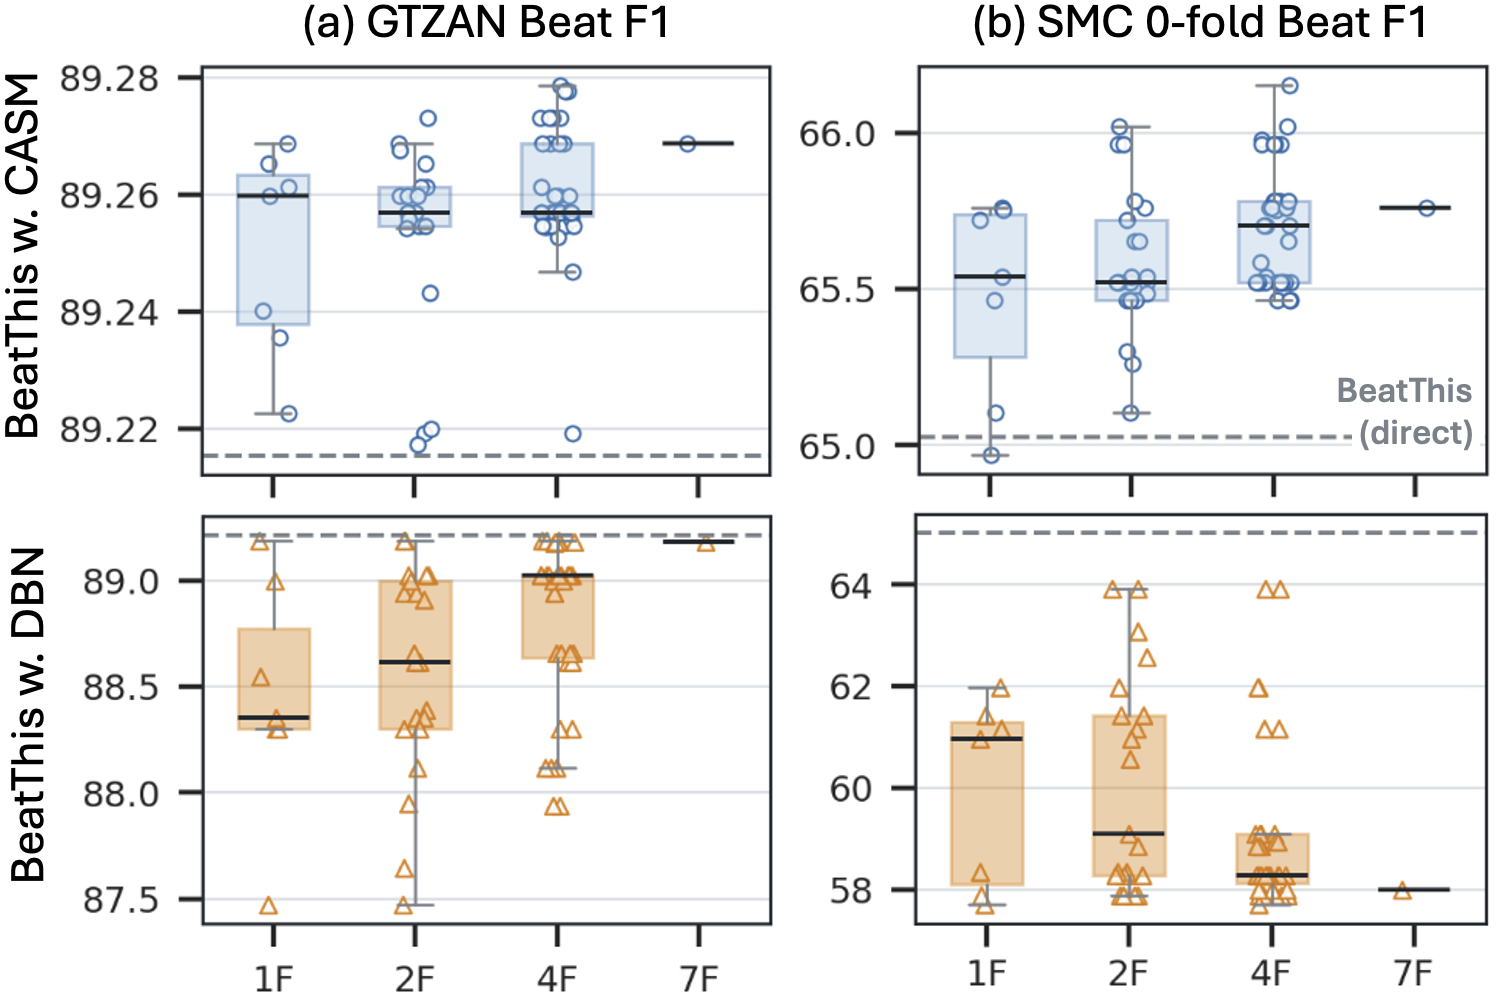
\includegraphics[width=0.9\columnwidth]{figures/p2.jpg}
\caption{Sensitivity to calibration data for CASM and DBN. Each point corresponds to a decoder configuration selected from one of the $7/21/35$ exhaustive 1-/2-/4-fold subsets of SMC folds 1--7 and evaluated on fixed SMC-fold-0 and GTZAN panels; 7F is a single configuration. Boxes are descriptive because calibration subsets overlap, and dashed lines show Direct performance.}
\label{fig:calibration-scale}
\end{center}
\end{figure}
\vspace{-3pt}
Fig.~\ref{fig:calibration-scale} shows a clear difference in calibration behaviour. CASM remains tightly clustered across fold combinations, and its central performance improves consistently as more calibration folds are used on both the held-out SMC panel and GTZAN. In contrast, DBN exhibits much wider variation across calibration subsets, and the trends on SMC and GTZAN do not move together: configurations favoured by one panel can transfer poorly to the other. This cross-dataset disagreement is consistent with stronger calibration-set over-specialisation in the fixed DBN parameterisation. The 7F CASM setting used in the main tables is therefore supported by the full available calibration pool rather than selected from a favourable smaller-fold combination.
\fi

\section{Conclusion and limitations}
\label{sec:concl}

CASM revisits structured beat decoding as an input-conditioned inductive bias rather than a return to one fixed tempo grid. It searches a sparse graph of activation maxima, centres each segment cost on a locally estimated period, and uses the period's margin over its strongest competitor to decide how strongly that cost should matter. Low margin softens the structured preference; only the independent count safeguard returns the exact Direct path. Once globally configured, the same deterministic module runs without upstream retraining, user annotation, or per-track BPM and meter input.

The present release verifies the frozen BeatThis--CASM pipeline, but does not yet support universal or three-backbone superiority claims: the controlled post-processor table and component ablations must be regenerated under one traceable frozen-7F protocol. Decoder calibration is also not strictly nested for the aggregate SMC estimate, and the existing CASM--DBN calibration-scale analysis uses unmatched selection pipelines. Future work should address these limitations with nested or leave-one-dataset-out calibration, matched-support baselines, explicit safeguard statistics, and additional frozen backbones. Multi-hypothesis period paths, causal decoding, and a differentiable duration layer are further methodological extensions.

\textbf{Acknowledgments.}
Computational resources were provided by the SongShan Lake HPC Center
(SSL-HPC) at Great Bay University.

\bibliographystyle{IEEEbib}
\bibliography{casm}

\end{document}
